% STL-Dev-MPI paper, first draft (A&A).
%
% Built with the A&A class 9.4 (aa.cls, aa.bst, from the A&A macro package
% of aanda.org, kept in this directory).  See README.md.
%
% Figures of the experiment are drawn at nside \nsidefig; switch it to 2048
% when the 2048 ensembles are measured (TODO_2048.md).  Lines whose numbers
% come from the nside 512 / 1024 ensembles carry the comment "% NUM2048".
\documentclass{aa}
\usepackage{graphicx}
\usepackage{amsmath}
\usepackage{xcolor}
\usepackage{url}
\usepackage{txfonts}
\usepackage{placeins}
\usepackage{tikz}
% Let the many full-width floats of Sect. 6 share pages (draft layout).
\renewcommand{\topfraction}{0.9}
\renewcommand{\dbltopfraction}{0.9}
\renewcommand{\textfraction}{0.07}
\renewcommand{\floatpagefraction}{0.75}
\renewcommand{\dblfloatpagefraction}{0.75}
\setcounter{topnumber}{3}
\setcounter{dbltopnumber}{3}

\newcommand{\nsidefig}{1024}
\newcommand{\todo}[1]{\textcolor{red}{[TODO: #1]}}
\newcommand{\nside}{N_{\rm side}}
\newcommand{\figfile}[2]{\IfFileExists{#1}{\includegraphics[width=#2]{#1}}{\fbox{\parbox{#2}{\centering\small missing figure \texttt{\detokenize{#1}}}}}}
\newcommand{\tabfile}[1]{\IfFileExists{#1}{\input{#1}}{\todo{missing table \texttt{\detokenize{#1}}}}}
\graphicspath{{figures/}}

\begin{document}

\title{Synthesising full-sky maps from scattering covariances on distributed-memory machines}
\subtitle{A pyramidal, block-wise explicit gradient in Rust, MPI and CUDA, applied to weak-lensing convergence}
\titlerunning{Scattering-covariance synthesis on distributed-memory machines}

% Authors: P. Campeti (first and corresponding author, finishes the study),
% J.-M. Delouis; further co-authors possible.  TODO: verify the affiliations.
% A&A 9.4: \corrauth for the corresponding author (footnote), \email{...}
% after each co-author (extracted by the editorial system, not printed),
% no ORCID; [longauth] only for long author lists.

\author{P. Campeti\inst{1}\corrauth{paolo.campeti@fe.infn.it}
  \and J.-M. Delouis\inst{2}\email{jean.marc.delouis@ifremer.fr}
  \and \todo{co-authors}}
\authorrunning{P. Campeti et al.}
\institute{INFN, Sezione di Ferrara, Ferrara, Italy \todo{verify affiliation}
  \and Laboratoire d'Oc\'eanographie Physique et Spatiale (LOPS), Univ. Brest, CNRS, Ifremer, IRD, Brest, France}
\date{Received ...; accepted ...}

\abstract
{Scattering-covariance statistics generate new realisations of a non-Gaussian field from one or a few examples with a small, interpretable set of constraints. On the sphere they are limited by the memory of automatic differentiation: a full-sky gradient at $\nside=2048$ ($5\times10^7$ pixels) fills a large GPU.}
{We make the synthesis scale with the nodes of a distributed-memory machine, each process holding a memory bounded by its share of the sky, and we test syntheses of a strongly non-Gaussian field against independent realisations.}
{The statistics and their exact gradient are computed without a computational graph, block by block, on a pyramid of anti-aliased HEALPix decimations; the cross-scale terms are carried by decimated moduli stored once per pair of levels, and blocks interact only through fixed halos. The Rust implementation uses MPI (contiguous NESTED ranges, halo exchanges, additive ghost cells, a distributed L-BFGS) and one CUDA device per rank, and matches the reference Python code to $10^{-15}$. For weak-lensing convergence the loss adds, in a gaussianised space, the first-order statistics of $\kappa$, the Wasserstein distance of the histogram, the power and the kurtosis of every pyramid level, and the scatter of an ensemble.}
{The evaluation time drops as the inverse of the number of ranks with 75--85\% efficiency up to 512 CPU cores at $\nside=1024$, with identical losses for any rank count. Ensembles of ten syntheses of the \citet{takahashi2017} convergence map at $\nside=1024$ lie within the scatter of ten independent realisations for the angular power spectrum, the per-level variance and kurtosis of $\kappa$ and the peak counts, but not for the Minkowski functionals of the finer levels. % NUM2048
\todo{2048 results.}}
{Scattering-covariance synthesis is no longer bound to the memory of one device, and the same machinery applies to high-resolution, multi-channel and time-dependent geophysical fields such as climate and ocean model outputs.}

\keywords{Methods: numerical -- Methods: statistical -- gravitational lensing: weak -- large-scale structure of Universe -- Techniques: image processing}

\maketitle

%======================================================================
\section{Introduction}
\label{sec:intro}

Many of the largest numerical data sets of the physical sciences are fields on the sphere. Kilometre-scale global climate and ocean models produce outputs of $10^7$ to $10^9$ cells per level and per variable, for many variables, every few hours over decades \citep{stevens2019,eyring2016,hewitt2020}; reanalyses such as ERA5 hold several decades of hourly global fields \citep{hersbach2020}; and the weather forecasts produced by machine-learning models are now judged as probabilistic ensembles of global fields \citep{lam2023,bi2023,price2025,kochkov2024}, some of them on HEALPix grids \citep{karlbauer2024}. In cosmology, wide surveys measure the weak-lensing convergence and the CMB on the full sky at arcminute resolution, and their non-Gaussian statistics are the target of a growing body of work \citep{kratochvil2010,kratochvil2012,petri2013,ajani2023,gatti2024}. All these applications need new realisations of the fields: to estimate covariances, to propagate uncertainties, to test pipelines, or to augment a small set of expensive simulations.

Generative models based on scattering transforms \citep{mallat2012,bruna2013} and their covariances \citep{morel2022,cheng2024} address this need with a different trade-off from deep generative networks. A scattering-covariance model describes a field by a few thousand averaged, interpretable coefficients that capture the coupling between scales and orientations; new realisations are drawn by gradient descent from noise until their coefficients match those of the data, in the spirit of microcanonical models \citep{bruna2019} and of texture synthesis \citep{portilla2000,gatys2015}. Such models need no training set: one realisation is enough \citep{allys2019,allys2020,cheng2020,cheng2021,jeffrey2022,regaldo2021}. They have been brought to the sphere for Planck dust polarisation \citep{delouis2022}, for astrophysical fields at large \citep{mcewen2022,mousset2024}, and to emulate CMB systematics from a handful of simulations \citep{campeti2025}.

The obstacle to larger maps is memory. The synthesis needs the gradient of the statistics with respect to every pixel. With automatic differentiation the computational graph keeps every intermediate field: on the sphere, the wavelet transforms of every scale and orientation, their moduli, and the second wavelet transforms of the moduli. The Python engine of STL-Dev\footnote{\url{https://github.com/STL-Proj/STL-Dev}} \citep{stldev} replaced the graph by an explicit, pyramidal and block-wise gradient, and synthesises an $\nside=2048$ map on one 24\,GB GPU. Beyond that size, and for several channels or for time sequences, one device is not enough, whatever the implementation.

This paper presents STL-Dev-MPI, a port of that engine to distributed-memory machines: Rust for the core, MPI for the decomposition of the sky between processes, and CUDA for one device per process. The memory of each process is bounded by its share of the sky; the wall-clock time per evaluation drops with the number of processes; and every rank count gives the same result to the last digits. We describe the method (Sect.~\ref{sec:method}), its parallel implementation on CPUs (Sect.~\ref{sec:mpi}) and GPUs (Sect.~\ref{sec:gpu}), and the terms we had to add to the loss to synthesise the weak-lensing convergence, a field whose information sits in rare, extended peaks (Sect.~\ref{sec:kappa}). We then test ensembles of ten syntheses of the \citet{takahashi2017} convergence map against the scatter of ten independent realisations of the same simulation suite, with statistics that are not in the loss: the angular power spectrum, the per-level variance and kurtosis, the peak counts, the one-point PDF and the Minkowski functionals (Sect.~\ref{sec:experiment}). Section~\ref{sec:outlook} discusses what the distributed implementation opens, in particular for climate and ocean data.

%======================================================================
\section{Method: a pyramidal, block-wise explicit gradient}
\label{sec:method}

A synthesis evaluates the statistics of a map and their gradient with respect to every pixel, hundreds of times. Two properties of the scattering covariance make this possible at any resolution. First, the gradient can be written by hand, family by family, and the intermediate fields it needs can be recomputed when they are needed instead of being stored: the memory of an evaluation is then that of the maps and of a few decimated fields, about 50 bytes per pixel at $L=4$, instead of the kilobytes per pixel that automatic differentiation keeps (Sects.~\ref{sec:ad} and \ref{sec:explicit}). Second, every operation of the statistics is local, except the final pixel means and the decimations that carry the fine moduli to the coarse levels, and both are sums: the statistics and their gradient are sums of contributions of blocks of pixels, each of which needs only the block and a thin halo around it (Sects.~\ref{sec:blocks} to \ref{sec:parallel}). The sky can then be split between processes like the grid of a finite-difference solver, and each process needs the memory of its share of the sky only.

\subsection{Scattering covariance on a HEALPix pyramid}
\label{sec:stats}

We use the scattering-covariance statistics of STL-Dev, which follow \citet{morel2022} and \citet{cheng2024} and were adapted to HEALPix \citep{gorski2005} by \citet{delouis2022} and \citet{mousset2024}; we only recall the notation. Let $x$ be a map at resolution $\nside$ (level 0) with $C$ channels, and $x_d = D^d x$ its anti-aliased decimations, level $d$ at $\nside/2^d$. One decimation step $D$ gives each coarse pixel a Gaussian-weighted, $\ell^1$-normalised mean of the fine pixels whose centres lie within $r = 3\,\theta_{\rm fine}$ of its centre ($\theta_{\rm fine}$ the fine pixel size, Gaussian width $r/2$). The wavelet $\psi$ is a complex directional filter with $L$ orientations, applied at every level with the same $K\times K$ stencil in the tangent plane (taps interpolated bilinearly from the four nearest pixels): $z_d = \psi\star x_d$ is a complex field of shape $[C, L, N_d]$, and scale $j$ is computed at level $d(j)=j$. Writing $\langle\cdot\rangle_n$ for a mean over the pixels of level $n$, the coefficients are
\begin{align}
S_1(j) &= \langle |z_{n}| \rangle_n, \qquad S_2(j) = \langle |z_{n}|^2 \rangle_n, \\
S_3(j_1,j_3) &= \langle [\psi\star m_{d_1,n}]_{\ell_1\ell_3}\; z^*_{n,\ell_3} \rangle_n, \\
S_4(j_1,j_2,j_3) &= \langle [\psi\star m_{d_1,n}]_{\ell_1\ell_3}\; [\psi\star m_{d_2,n}]^*_{\ell_2\ell_3} \rangle_n,
\end{align}
with $n=d(j_3)$ ($n=d(j)$ for $S_1$, $S_2$), $d_i = d(j_i)$, cross-channel versions of each, the mean and variance of the map, and the \emph{stored moduli}
\begin{equation}
m_{d,n} = D^{\,n-d}\,|z_d| \qquad (d<n),
\label{eq:moduli}
\end{equation}
the modulus of the wavelet field of level $d$ decimated to level $n$. Every coefficient is a pixel mean at its \emph{native level} $n$. With $L=4$, $K=5$ and $J=\log_2\nside-1$ scales, a single-channel map has 11\,354 coefficients at $\nside=1024$ and 15\,042 at 2048.

The synthesis minimises over the map $x$
\begin{equation}
\mathcal{L}_S(x) = \frac{1}{N_c}\sum_{i} \frac{|S_i(x) - S_i(t)|^2}{\sigma_i^2}, \qquad \sigma_i^2 = \frac{\langle |f_{i}|^2\rangle - |S_i(t)|^2}{N_{n(i)}},
\label{eq:loss}
\end{equation}
with $t$ the target, $f_i$ the field whose mean is $S_i$, and $N_{n}$ the number of pixels of level $n$: $\sigma_i^2$ is the variance of a mean of $N_n$ independent pixels, estimated on the target (ergodic hypothesis), and $\mathcal{L}_S$ is a reduced $\chi^2$. Without these weights the loss is dominated by the low-order coefficients and $S_3$, $S_4$ stay at 1--3$\sigma$ after 400 iterations; with them every family converges below $1\sigma$.

\subsection{What automatic differentiation stores}
\label{sec:ad}

The earlier syntheses on the sphere \citep{delouis2022,mousset2024} obtain the gradient from the automatic differentiation of a machine-learning framework, PyTorch \citep{paszke2019} or JAX \citep{jax2018}. In reverse mode, every operation of the forward computation records the inputs that its derivative needs, and the record is kept until the backward pass has used it. For the statistics of Sect.~\ref{sec:stats} the record holds at least, for every level $n$: the wavelet fields $z_n$ and their moduli ($\frac{4}{3}LN$ complex and $\frac{4}{3}LN$ real values over the pyramid, for a map of $N$ pixels and one channel); the decimation chains of the moduli; and the second wavelet fields $\psi\star|z_n|$ and $\psi\star m_{d,n}$ for every finer level $d<n$ and every pair of orientations, $(n+1)L^2$ complex fields of $N_n = N/4^n$ pixels at level $n$, $\frac{16}{9}L^2N$ complex values in all, which alone is 455 bytes per pixel of the map at $L=4$. Actual implementations record more (normalised fields, gathered convolution taps, intermediate products), and the convolution geometry (the rotated stencil of every pixel and its interpolation weights) is usually precomputed for the whole sky and kept. In STL-Dev, the automatic-differentiation version of the same statistics holds 371\,MB of graph for a map of 49\,152 pixels ($\nside=64$, $J=5$, $L=2$, $K=5$), 7.5\,kB per pixel, on top of a stored geometry of 3.2\,kB per pixel \citep{stldev}. Both grow in proportion to the number of pixels: at $\nside=2048$ ($5\times10^7$ pixels) the graph would take about 380\,GB at $L=2$, more at $L=4$, and the geometry 160\,GB. This, and not the arithmetic, is what has limited the syntheses to one device and to moderate resolutions.

\subsection{An explicit gradient}
\label{sec:explicit}

Every coefficient is the pixel mean, at its native level, of a product of two fields, $S=\langle a\,b^*\rangle_n$, or of a modulus. Its derivative is known in closed form: a cotangent on $S$ gives, pixel by pixel, a cotangent on $a$ proportional to $b$ and a cotangent on $b$ proportional to $a$, both divided by $N_n$. The chain then runs backwards through operations whose adjoints are explicit and sparse: the second wavelet convolution (its adjoint scatters every interpolated tap back to the four pixels it came from), the decimations ($D^\top$), the modulus ($\bar z = \overline{|z|}\,z/|z|$), the first wavelet convolution, and finally the decimations that made $x_n$ from $x$. Each adjoint costs about as much as the operation itself; the gradient is checked against finite differences, and the explicit gradient of the reference against its automatic differentiation (Table~\ref{tab:validation}).

The fields that the backward pass needs are not kept: they are recomputed from the maps when the backward pass reaches them, block by block (Sect.~\ref{sec:sweeps}). This is the checkpointing strategy of automatic differentiation pushed to its limit, and it costs one extra evaluation of the forward fields. Only two kinds of quantities must survive from the forward to the backward pass, because they cannot be recomputed locally: the maps of all levels, $x_d=D^dx$ ($\frac{4}{3}N$ values per channel), and the stored moduli $m_{d,n}$ of Eq.~(\ref{eq:moduli}). The stored moduli are the only carriers of information across scales: $S_3$ and $S_4$ at level $n$ read the moduli of all the finer levels, but only after their decimation to level $n$, which divides their size by $4^{n-d}$. Summed over the pairs $d<n$, they hold $\frac{4}{9}LN$ values per channel, less than the moduli of the finest level alone. With the cotangents of both, the state of an evaluation is $2(\frac{4}{3}+\frac{4}{9}L)NC$ real values, 50 bytes per pixel and map at $L=4$, against the 7.5\,kB per pixel of graph and 3.2\,kB per pixel of geometry above. The convolution geometry is recomputed for each block and never stored (Sect.~\ref{sec:memory}).

\subsection{Locality and blocks}
\label{sec:blocks}

Every operation of the chain is local. A wavelet convolution reads the $K\times K$ stencil of a pixel, each tap interpolated from its four nearest pixels; a decimation step reads the fine pixels within $r=3\,\theta_{\rm fine}$ of a coarse centre; moduli and products act pixel by pixel. A field on a set $F$ of pixels of level $n$ therefore needs its inputs only on $F$ plus a \emph{halo} of a few pixels of that level, whatever the size of the map. Only two operations are not local, and both are sums. The coefficients are pixel means: they are sums of partial sums over any partition of the native level into blocks. The stored moduli carry $|z_d|$ across $n-d$ levels; since $D$ is linear,
\begin{equation}
m_{d,n} = \sum_k D^{\,n-d}\left(|z_d|\,\mathbf{1}_{F_k}\right),
\label{eq:pieces}
\end{equation}
where $\{F_k\}$ is a partition of level $d$ into blocks of $b$ pixels. Each \emph{piece} needs $z_d$ on $F_k$ only, which needs $x_d$ on $F_k$ plus a convolution halo, and its decimation chain is supported on a cone that grows by a decimation halo per level (Fig.~\ref{fig:blocks}). The gradient goes back through the transposed pieces, the derivative of the modulus and the adjoint of the wavelet convolution, on the same supports.

Halos are counted in pixels of their level: $(K-1)/2 + 2$ for a convolution, $\lceil r/\theta\rceil + 1$ for a decimation, doubled for the pieces and their transposes so that every coarse row touched by a block sees its whole cone. Fine-level dilations are computed at the parent level ($k$ coarse rings cover at least $2k$ fine pixels). The blocks are NESTED ranges, compact on the sphere, so a halo is a thin ring around a patch.

The statistics are thus a sum over blocks of partial sums, each computed from the block and its halo, and the gradient, which runs the same chain backwards, is a sum over blocks of contributions, each written into the block and its halo. Between two blocks nothing is kept but the maps, the stored moduli and their cotangents: the fields of a block, $z_n$, its modulus and the second wavelets on $F$ plus a halo, have a size set by $b$, not by $N$. The result does not depend on the blocks: any $b$, from 64 pixels to whole levels, gives the full-sky statistics and gradient to rounding (Sect.~\ref{sec:validation}).

\begin{figure*}
\centering
\resizebox{0.95\textwidth}{!}{%
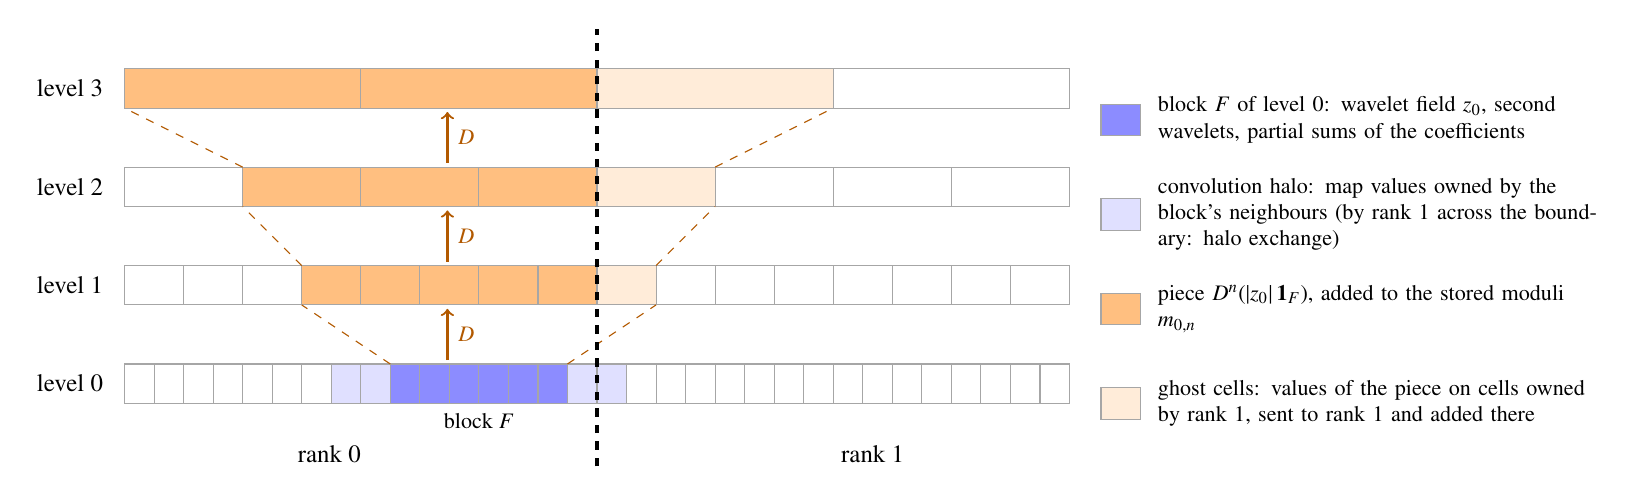
\begin{tikzpicture}[font=\small]
\def\H{1.25}
\fill[blue!12] (2.625,0) rectangle (3.375,0.5);
\fill[blue!12] (5.625,0) rectangle (6.375,0.5);
\fill[blue!45] (3.375,0) rectangle (5.625,0.5);
\fill[orange!50] (2.25,{\H}) rectangle (6,{\H+0.5});
\fill[orange!15] (6,{\H}) rectangle (6.75,{\H+0.5});
\fill[orange!50] (1.5,{2*\H}) rectangle (6,{2*\H+0.5});
\fill[orange!15] (6,{2*\H}) rectangle (7.5,{2*\H+0.5});
\fill[orange!50] (0,{3*\H}) rectangle (6,{3*\H+0.5});
\fill[orange!15] (6,{3*\H}) rectangle (9,{3*\H+0.5});
\foreach \d/\n in {0/31,1/15,2/7,3/3}{
  \pgfmathsetmacro{\w}{0.375*2^\d}
  \foreach \i in {0,...,\n}{\draw[gray!70] ({\i*\w},{\d*\H}) rectangle ++(\w,0.5);}
  \node[anchor=east] at (-0.15,{\d*\H+0.25}) {level \d};
}
\draw[dashed,orange!70!black] (3.375,0.5) -- (2.25,{\H}) (2.25,{\H+0.5}) -- (1.5,{2*\H}) (1.5,{2*\H+0.5}) -- (0,{3*\H});
\draw[dashed,orange!70!black] (5.625,0.5) -- (6.75,{\H}) (6.75,{\H+0.5}) -- (7.5,{2*\H}) (7.5,{2*\H+0.5}) -- (9,{3*\H});
\foreach \d in {0,1,2}{\draw[->,thick,orange!70!black] (4.1,{\d*\H+0.55}) -- node[right,font=\footnotesize]{$D$} (4.1,{(\d+1)*\H-0.05});}
\draw[very thick,dashed] (6,-0.8) -- (6,{3*\H+1.0});
\node[below,font=\footnotesize] at (4.5,0) {block $F$};
\node at (2.6,-0.65) {rank 0};
\node at (9.5,-0.65) {rank 1};
\foreach \c/\t [count=\k] in {blue!45/{block $F$ of level 0: wavelet field $z_0$, second wavelets, partial sums of the coefficients},
  blue!12/{convolution halo: map values owned by the block's neighbours (by rank 1 across the boundary: halo exchange)},
  orange!50/{piece $D^{n}(|z_0|\,\mathbf{1}_F)$, added to the stored moduli $m_{0,n}$},
  orange!15/{ghost cells: values of the piece on cells owned by rank 1, sent to rank 1 and added there}}
{\fill[\c] (12.4,{4.6-1.2*\k}) rectangle ++(0.5,0.4);
 \draw[gray!70] (12.4,{4.6-1.2*\k}) rectangle ++(0.5,0.4);
 \node[anchor=west,text width=5.6cm,font=\footnotesize] at (13.0,{4.8-1.2*\k}) {\t};}
\end{tikzpicture}}
\caption{Locality of the statistics, in one dimension (a cartoon of the sphere, where each level has four times fewer pixels than the level below). The wavelet field of a block $F$ of level 0 needs the map on $F$ and a convolution halo. Its modulus restricted to $F$ is decimated level by level (the piece of Eq.~\ref{eq:pieces}), on a support that grows by a decimation halo per level (dashed), and is added to the stored moduli. With the sky split between processes, a halo cell owned by another process is filled by a halo exchange, and a piece's values on cells owned by another process are sent to it and added (ghost reduction). The gradient runs the same supports backwards: transposed pieces, modulus derivative, convolution adjoint.}
\label{fig:blocks}
\end{figure*}

\subsection{Sweeps}
\label{sec:sweeps}

One evaluation of the loss and of its gradient is two sweeps over the levels.

\emph{Upward sweep}, $n = 0, \dots, J-1$: for every block $F$ of level $n$, (i) the wavelet field $z_n$ on $F$ plus a halo, from $x_n$ on $F$ plus two halos; (ii) the second wavelets of $|z_n|$ (same level) and of $m_{d,n}$ ($d<n$, read from the stored maps) on $F$; (iii) the partial sums of every coefficient of native level $n$; (iv) the piece $|z_n|\mathbf{1}_F$ pushed down to every coarser level $n'>n$ and added to $m_{n,n'}$.

\emph{Downward sweep}, $n = J-1, \dots, 0$: for every block of level $n$, the fields of the upward sweep are recomputed; the coefficient cotangents $2(S_i - S_i(t))/(N_c\sigma_i^2)$ (real and imaginary parts for complex coefficients) are applied; the cotangents $g_{d,n}$ of the stored moduli of the finer levels are accumulated (they are complete once the coarser levels are done); the block's own chain is reversed from $g_{n,n'}$, $n'>n$, through the transposed pieces; then the modulus derivative and the wavelet adjoint give the cotangent of $x_n$ on the block.

Finally the map cotangents of all levels are brought back to level 0 by Horner's scheme through the transposed decimations, $\nabla_x\mathcal{L} = \sum_d (D^\top)^d\,g_{x_d}$. Everything is in double precision and every summation order is fixed.

\subsection{Why the gradient parallelises}
\label{sec:parallel}

Locality turns the gradient into a domain-decomposition problem, like the solution of a partial differential equation on a grid. Let the pixels of level 0 be split between $P$ processes as compact patches, each process owning the parents of its pixels at every level. A process can compute the contributions of all its blocks, in both sweeps, if it holds at every level its own pixels plus a ring of halo pixels, and if it knows the cotangents of the $N_c$ coefficients, which are global. Three kinds of communication are enough (Sect.~\ref{sec:mpi}): halo exchanges, which copy into the ring the values owned by the neighbouring processes (maps, stored moduli, cotangents); ghost reductions, which send the contributions that a process wrote into its ring (the edges of its pieces and of its transposed convolutions) to their owners, where they are added; and one global sum of the $N_c$ partial sums per evaluation, after which every process knows the statistics, the loss and the cotangents of the coefficients. Nothing else couples distant pixels.

Three consequences follow. (i) The memory of a process is its share of the state of Sect.~\ref{sec:explicit}, $(50 + 192)\,N/P$ bytes at $L=4$ with the L-BFGS history, plus its halo ring and the transients of one block. The ring scales as the perimeter of the patch: at $\nside=1024$ on 64 processes a process owns 196\,608 pixels of level 0 and holds 13\% more with its halos (Sect.~\ref{sec:performance}). (ii) The communication of a process also scales as its perimeter, $\propto(N/P)^{1/2}$ at fixed level, plus a vector of $N_c$ coefficients, independent of $N$. (iii) There is no limit on the size of the map other than the number of processes: multiplying $N$ by four (one more level of $\nside$) with four times as many processes leaves the memory and the work of each process unchanged. A synthesis that does not fit one device runs on several, with the same result to rounding: $\nside=2048$ at $L=4$ does not fit one 16\,GB GPU but runs on two, and $\nside=4096$ runs on 16 GPUs of 16\,GB (Sect.~\ref{sec:gpu}). The coarsest levels hold fewer pixels than there are processes, so their halos may cover them entirely; they are small ($N/4^d$ pixels), and holding them in full costs little. Since the global sums are made in a fixed rank order, the result does not depend on $P$.

\subsection{Memory}
\label{sec:memory}

Per block the engine holds fields of size $|F + {\rm halo}|$ times $C L$, and the convolution geometry of the block's rows: the rotated stencil of each output row, interpolated on the four nearest pixels, $4GK^2$ entries per row for $G$ gauges, computed on the fly and never stored globally (a stored geometry costs kilobytes per pixel). Globally it holds the maps of all levels and their cotangents ($2\times\frac{4}{3}NC$ values), the stored moduli and their cotangents ($2\times\frac{4}{9}NCL$, real), and the history of L-BFGS ($2(h+2)N$ values for a history $h$, work vectors included). For $B$ maps synthesised together, every term is multiplied by $B$. At $L=4$ and $C=1$ the maps, the stored moduli and their cotangents take $8(8/3+8L/9)\simeq50$ bytes per pixel and map before the halos (0.6\,GB at $\nside=1024$, 2.5\,GB at 2048), and L-BFGS with $h=10$ adds 192 bytes per pixel and map. The GPU engine (Sect.~\ref{sec:gpu}) also keeps the level fields $z_n$ and $|z_n|$ whole, about 220 bytes per pixel and map in all (2.8\,GB at $\nside=1024$, 11.1\,GB at 2048). The point of the decomposition (Sect.~\ref{sec:mpi}) is that all these terms are divided by the number of processes.

\subsection{Validation against the reference}
\label{sec:validation}

STL-Dev-MPI was written against fixtures dumped from STL-Dev; every test compares the two (Table~\ref{tab:validation}). The geometry agrees to $10^{-12}$ or to the rounding of the reference itself (its \texttt{acos} differs from the C library's by one ulp on about 10\% of the inputs, amplified by $1/\sin\theta$ near the poles). The statistics agree to $7\times10^{-16}$ and the gradients to $9\times10^{-16}$, over 8 cases with $\nside=16$ and 32, $J=3$ and 4, $L=2$ and 4, kernels 3 and 5, 1 and 2 channels, both definitions of $S_3$/$S_4$, and blocks from 64 pixels to whole levels. The L-BFGS optimiser is a line-by-line port of \texttt{torch.optim.LBFGS} \citep{liu1989,paszke2019} with its strong Wolfe line search \citep{wolfe1969,nocedal2006}: a 20-iteration synthesis of the WebSky convergence map at $\nside=64$ reproduces the 25 loss values of STL-Dev at the printed precision, with any number of ranks.

\begin{table}
\caption{Agreement of STL-Dev-MPI with the STL-Dev reference.}
\label{tab:validation}
\centering\small
\begin{tabular}{lr}
\hline\hline
Quantity & Max.\ difference \\
\hline
Pixel indices, neighbours, decimation sparsity & exact \\
Pixel centres, stencil rotations & $10^{-14}$ \\
Ring interpolation, decimation weights & $10^{-12}$ \\
Block wavelet, adjoint, pieces & $8\times10^{-14}$ \\
Statistics (values $O(1)$) & $7\times10^{-16}$ \\
Map and band gradients & $9\times10^{-16}$ \\
Gradient vs finite differences (relative) & $2.5\times10^{-9}$ \\
2, 4 ranks vs 1 (threads, \texttt{mpirun}) & $7\times10^{-16}$ \\
GPU vs CPU statistics & $6\times10^{-16}$ \\
L-BFGS losses vs STL-Dev$^a$ & $2.3\times10^{-10}$ \\
\hline
\end{tabular}
\tablefoot{$^a$ $\nside=64$, 25 evaluations.}
\end{table}

%======================================================================
\section{Distributed memory}
\label{sec:mpi}

\subsection{Decomposition and halos}

The sky at level 0 is split into contiguous NESTED ranges, one per rank, aligned on $4^k$ pixels with $k$ as large as the rank count allows. A rank owns the cell $c$ of level $d$ when its first descendant at level 0, $c\,4^d$, is in its range. When the ranges are aligned on $4^{J-1}$, every rank owns the parents of all its cells and its pyramid is aligned: $x_d$, $m_{d,n}$ and their cotangents are sliced the same way at every level. With more ranks than cells at the coarsest levels, some ranks own no coarse cell; nothing else changes.

Each rank holds, at every level, its owned cells plus the halo cells that its blocks touch: the convolution domains of its blocks, the decimation domains of the blocks of the next level, the parents of its cells, and the supports of the decimation chains of its finer blocks (Sect.~\ref{sec:blocks}). These layouts are computed once. The neighbours are found with HEALPix neighbourhoods at the parent level, and each rank tells the owners of its halo cells which cells it needs; the counts on both sides are checked once at set-up.

Two kinds of exchange cross rank boundaries during the sweeps \citep[the ghost-cell pattern of domain decomposition;][]{smith1996}: \emph{halo exchanges}, where owners send the current values of the cells their neighbours hold (maps after each decimation, stored moduli before they are read, cotangents before the transposed decimations), and \emph{ghost reductions}, where the contributions that a rank's pieces and transposed pieces wrote into cells owned by a neighbour are sent to the owner and added. Owners add the contributions of the other ranks in rank order, so the result does not depend on the arrival order of the messages. Both are point-to-point messages with neighbours only, one tag per exchange; the exchanges of all the stored moduli of a level are batched, so an evaluation needs about $5L$ exchanges with each neighbour (26 at $\nside=64$, about 56 at 2048, instead of 58 and 218 before batching). The partial sums of the coefficients are gathered and broadcast in rank order (one vector of $N_c$ complex numbers per evaluation), so that the statistics, the loss and every decision of the optimiser are identical on every rank and do not depend on the number of ranks: 1, 2 and 4 ranks agree to $7\times10^{-16}$, and the $\nside=1024$ runs of Table~\ref{tab:cpu} on 24 to 192 ranks and 1 to 4 nodes give the same losses to 16 digits.

No rank ever holds a full-sky map: the target and the initial map are read by owned slices, the white noise of the initial map is drawn per pixel from (seed, pixel) so that it does not depend on the decomposition, and the outputs are written by slices at their offsets.

\subsection{Distributed L-BFGS}

The L-BFGS history vectors are distributed like the map. The two-loop recursion and the strong Wolfe line search need only dot products and norms, which are global sums of per-rank partial sums (in rank order). The port of \texttt{torch.optim.LBFGS} goes through an abstract reduction, so the same code runs on one process, on thread ranks (for the tests), and under MPI.

\subsection{Ensembles}
\label{sec:ensembles}

An ensemble of $B$ syntheses is optimised jointly with the loss on the mean of their statistics,
\begin{equation}
\mathcal{L}_S = \frac{1}{N_c}\sum_i \frac{|\bar S_i - S_i(t)|^2}{\sigma_i^2/B}, \qquad \bar S_i = \frac{1}{B}\sum_{m=1}^{B} S_i(x_m),
\label{eq:ensemble}
\end{equation}
so that the ergodic scatter of the target goes into the differences between the members instead of being forced to zero in each of them. The mean alone leaves the scatter free (at $\nside=64$ every member of a 4-member ensemble ends 3--4.6$\sigma$ from the target, where an ergodic realisation sits about $1\sigma$ away); a second-moment term holds it at the ergodic variance:
\begin{equation}
\mathcal{L}_D = \frac{w_D}{N_c}\sum_i\left(\frac{\mathcal{D}_i}{\sigma_i^2}-1\right)^2, \qquad \mathcal{D}_i = \frac{1}{B-1}\sum_m |S_i(x_m) - \bar S_i|^2.
\label{eq:scatter}
\end{equation}
With $w_D=1$ the members end at about $1\sigma$ from the target, with a scatter at the ergodic variance (0.94--1.12 per family at $\nside=64$).

The ranks are split into $G$ groups of consecutive ranks (\texttt{MPI\_Comm\_split}); a group shares the sky of $B/G$ members, which its engine evaluates as a batch, and the groups exchange one vector of $N_c$ complex partial sums (and one of $N_c$ reals for Eq.~\ref{eq:scatter}) per evaluation. $G=1$ costs no extra communication and suits small maps; $G=B$ gives each member the memory and time of a single synthesis on $P/B$ ranks or devices. Any $G$ gives the same synthesis up to the order of the sums ($10^{-12}$ relative after 30 iterations at $\nside=64$).

\subsection{Overlap mode}

An alternative decomposition (option \texttt{-{}-overlap}, CPU engine) trades computation for communication. Every rank evaluates, for the fine levels ($d < n_c$), its owned blocks and the halo blocks they depend on, on extended regions, so that the sweeps need no exchange; the coarse levels ($d\geq n_c$), small, are held whole and evaluated by rank 0. An evaluation then needs only the level-0 map halo, one global sum of the coarse stored moduli and of the map of level $n_c$, the coefficient sum, one broadcast of the coarse cotangents and the level-0 ghost reduction of the map cotangent. It agrees with the standard mode to $7\times10^{-16}$ on every fixture with 1, 2 and 4 ranks. \todo{timings of the overlap mode at scale.}

\subsection{Performance}
\label{sec:performance}

Table~\ref{tab:cpu} and Fig.~\ref{fig:scaling} give the time of one evaluation (statistics and gradient) on three clusters: Datarmor (Ifremer; $2\times$ Xeon E5-2680 v4 per node, Intel MPI), the hpc cluster ($2\times$ AMD EPYC 9655 per node, OpenMPI 5) and Ir\`ene Rome (TGCC; AMD EPYC 7H12, OpenMPI 4.1). At $\nside=64$ the time drops by 10 at 28 ranks on Datarmor and by 11.5 at 128 ranks on hpc, where it saturates (a rank owns 384 pixels of level 0 at 128 ranks). At $\nside=1024$ the efficiency is 75\% from 24 to 192 ranks on one hpc node, and spreading the 192 ranks over 4 nodes costs 5\%; on Ir\`ene it is 85\% from 128 to 512 ranks. $L=4$ costs 1.3 to 1.5 times $L=2$ (12.8\,s per evaluation on 512 Ir\`ene ranks at $\nside=1024$, 33.1\,s on 160 ranks). Ensembles add the members' work and one exchange of partial sums between groups: a production ensemble of 10 maps at $\nside=1024$, $L=4$, with all the terms of Sect.~\ref{sec:kappa}, runs at 128.4\,s per evaluation (all members) on 640 Ir\`ene cores in 10 groups of 64 (316 evaluations in 11.3\,h, the loss going from $5.7\times10^4$ to 2.46); the same ensemble without the $\kappa$ terms ran at 149\,s on 160 hpc cores in 10 groups of 16. The state per rank (maps, stored moduli, cotangents, L-BFGS history) shrinks as $1/P$: 123\,MB at 24 ranks, 17\,MB at 192 for $\nside=1024$, $L=2$. In the Ir\`ene ensemble a rank owns 196\,608 cells of level 0 and holds 221\,760 with its halos; its state is 52.5\,MB, of which 37.7\,MB of L-BFGS history, 9.7\,MB of stored moduli and cotangents and 5.1\,MB of maps and cotangents (the halos weigh most on the stored moduli, which live on the coarse levels). What remains is the transients of one block (80--160\,MB for blocks of 16\,384 pixels, halved with blocks of 4096) and the MPI runtime (20--30\,MB per rank for Intel MPI, 200--350\,MB for OpenMPI~5). For comparison (on another machine), STL-Dev on the $\nside=64$ case takes 12.6 to 18\,s per evaluation on 4 CPU threads with a peak of 1.9\,GB, against 8.1\,s and 103\,MB for one STL-Dev-MPI rank on Datarmor.

\begin{figure*}
\centering
\figfile{figures/scaling.pdf}{0.95\textwidth}
\caption{Strong scaling of one evaluation (statistics and gradient). (a) $\nside=64$, $L=2$, on Datarmor and hpc; (b) $\nside=1024$, $L=2$, on one hpc node and on Ir\`ene Rome; (c) $L=4$ on one to three Tesla T4 GPUs (garoupe) at $\nside=256$, 1024 and 2048 (one T4 cannot hold $\nside=2048$). Dashed lines: ideal scaling from the first point.}
\label{fig:scaling}
\end{figure*}

\begin{table}
\caption{Seconds per evaluation on CPUs (kernel 5, blocks of 16\,384 pixels, one map).}
\label{tab:cpu}
\centering\small
\begin{tabular}{rrrlr}
\hline\hline
$\nside$ & $L$ & Ranks & Machine & s / eval. \\
\hline
64 & 2 & 1 & Datarmor & 8.06 \\
64 & 2 & 28 & Datarmor & 0.81 \\
64 & 2 & 1 & hpc & 3.26 \\
64 & 2 & 128 & hpc & 0.28 \\
1024 & 2 & 24 & hpc, 1 node & 60.9 \\
1024 & 2 & 192 & hpc, 1 node & 10.2 \\
1024 & 2 & $4\times48$ & hpc, 4 nodes & 10.6 \\
1024 & 2 & 128 & Ir\`ene Rome & 30.2 \\
1024 & 2 & 512 & Ir\`ene Rome & 8.9 \\
1024 & 4 & 512 & Ir\`ene Rome & 12.8 \\
1024 & 4 & 160 & \todo{machine} & 33.1 \\
\hline
\end{tabular}
\end{table}

%======================================================================
\section{GPU engine}
\label{sec:gpu}

The GPU engine runs the same sweeps on one CUDA device per MPI rank, with the CPU decomposition, exchanges, objective and L-BFGS. Its kernels are compiled at start-up by NVRTC to a native binary for the device, with fused multiply-adds disabled and IEEE division and square root, and loaded through the \texttt{cudarc} crate \citep{cudarc}, so the code builds without a CUDA toolkit. Every expression is evaluated in the order of its CPU counterpart, there are no floating-point atomics, and the results are identical from run to run; they differ from the CPU engine only through the transcendental functions and a few documented summation orders (statistics within $6\times10^{-16}$, level-0 gradient within $9\times10^{-13}$ of its maximum). With one rank, nothing leaves the device; with several, the halo cells are exchanged through the host.

\emph{Blocks and geometry.} On the device a level is processed by blocks of up to $2^{20}$ owned cells, sized from the free memory, hundreds of times larger than on the CPU; the layouts do not depend on the block size, so device blocks read the same halos. The convolution geometry (rotated stencils, ring bilinear interpolation, binding to the rank's grid) is computed by a kernel per output row and gauge, then transposed by grid cell so that the adjoint convolution is a gather in a fixed order. Within a memory budget, the geometry of the blocks is kept between sweeps either whole (24 bytes per entry) or as its transposition only (4 bytes per entry, the weights being recomputed).

\emph{Decimations.} Instead of pieces, the device applies the full-sky decimation rows of the rank's owned coarse cells to the halo-exchanged finer field; the reverse chain is accumulated from the coarsest level by Horner's scheme. These are the values of the pieces, summed in another order.

\emph{One engine per rank.} A synthesis evaluates several objectives on the same decomposition: the target statistics, the synthesis itself and, for weak lensing (Sect.~\ref{sec:kappa}), the statistics of $\kappa=f(g)$. One engine per rank is shared by all of them (topology, decimation rows, geometry cache and level fields), since an evaluation of one objective ends before the next starts. A plan without $S_3$ or $S_4$ neither computes nor allocates the moduli, the stored moduli and their chains. The level fields of the full plan then take $8BCH_0(8/3 + 56L/9)$ bytes for $H_0$ cells held at level 0 and $B$ members, and the geometry cache takes most of what remains. Before this change, a 10-member ensemble at $\nside=1024$ with the $\kappa$ term did not fit on one 141\,GB H200 without capping the geometry caches; on a 6\,GB laptop GPU, a 2-member ensemble at $\nside=128$ with the $\kappa$ term, which needed such a cap, now runs 2.6 times faster per evaluation, with identical losses.

\emph{Performance} (Table~\ref{tab:gpu}). On the Tesla T4, whose double-precision throughput is 1/32 of its single precision, three devices take 13.3\,s per evaluation at $\nside=1024$, $L=4$, and 114\,s at 2048, where the geometry no longer fits and is rebuilt at each sweep; three T4s are twice as fast as a 192-core EPYC node at $\nside=1024$, $L=2$. The scaling from 1 to 3 T4s is superlinear while the geometry cache covers more of each rank's rows. On H200 GPUs, an ensemble of 10 syntheses at $\nside=1024$ runs on a single device, and a single map at $\nside=4096$ ($2\times10^8$ pixels, $J=11$) takes about 325\,s per evaluation on one device and 67.9\,s on two, a superlinear gain as on the T4s, where it comes from the geometry cache covering more of each rank's rows. The same $\nside=4096$ synthesis runs on 16 V100s with 16\,GB each (25.2\,s per evaluation, 13.9\,GB per device): small devices are usable as long as there are enough of them. On Ir\`ene, a node of 4 V100s is worth about 1024 AMD Rome cores (23.4 against 28.8\,s per evaluation for the same synthesis at $\nside=2048$).

\begin{table}
\caption{Seconds per evaluation on GPUs ($L=4$, kernel 5, double precision). $B$: maps synthesised together; ``mem.'': device memory peak per GPU, cache included.}
\label{tab:gpu}
\centering\small
\begin{tabular}{rrlrrr}
\hline\hline
$\nside$ & $B$ & GPUs & s / eval. & mem.\ (GB) \\
\hline
256 & 1 & 1 T4 & 1.26 & 9.1 \\
256 & 1 & 3 T4 & 0.34 & 4.0 \\
1024 & 1 & 1 T4 & 66.8 & 12.3 \\
1024 & 1 & 3 T4 & 13.3 & 10.9 \\
2048 & 1 & 2 T4 & 474 & 13.8 \\
2048 & 1 & 3 T4 & 114 & 12.9 \\
512 & 10$^a$ & 2 T4 & 50.6 & 13.3 \\
1024 & 10$^a$ & 1 H200 & 54.3 & 98 \\
2048 & 5$^a$ & 1 H200 & 157 & 139 \\
4096$^b$ & 1 & 1 H200 & $\sim$325 & -- \\
4096$^b$ & 1 & 2 H200 & 67.9 & 124 \\
4096$^b$ & 1 & 16 V100 & 25.2 & 13.9 \\
\hline
\end{tabular}
\tablefoot{$^a$ Ensembles with the $\kappa$ terms of Sect.~\ref{sec:kappa}. $^b$ Synthesis of the $\nside=2048$ convergence map at twice its resolution ($J=11$, 19\,450 coefficients); the H200 memory is mostly geometry cache, which fills the device. T4: garoupe; H200: hpc cluster; V100: Ir\`ene (4 nodes of 4 V100 16\,GB, job 6048940).}
\end{table}

%======================================================================
\section{Synthesising the weak-lensing convergence}
\label{sec:kappa}

\subsection{Gaussianised synthesis}

The convergence $\kappa$ at low source redshift is dominated by rare, extended haloes: the map used below has a skewness of 8.4 at $\nside=64$. Synthesising $\kappa$ directly works poorly, and we synthesise its Gaussian anamorphosis instead, as in FOSCAT \citep{foscat}: the pixel of rank $r$ among $N$ becomes $g = \Phi^{-1}((r+1/2)/N)$, and a synthesis $g$ is mapped back by matching the target's histogram. Three choices made the synthesis of $g$ reliable:
\begin{itemize}
\item \emph{$L=4$ orientations.} With $L=2$ the syntheses are elongated east--west (east--west to north--south small-scale power 0.89$\pm$0.03 against 1.02$\pm$0.05 for the target at $\nside=256$).
\item \emph{Coarse to fine.} Each resolution starts from the previous one replicated on the children, plus white noise with the rms of the target's scales missing at the coarser resolution; ensembles carry each member to the next resolution.
\item \emph{Power of every pyramid level.} The scattering coefficients leave the finest scale loose: with every family below $0.5\sigma$, a synthesis at $\nside=256$ holds only 58\% of the variance of the finest details. Writing $d_n$ for the details of level $n$ (the map at $\nside=n$ minus the mean of each group of four children) and $V_n$ for their variance, we add
\begin{equation}
\mathcal{L}_P = \frac{w_P}{B}\sum_m\sum_n\left(\frac{V_n(g_m)}{V_n(t)}-1\right)^2,
\end{equation}
with its exact gradient; at $w_P=1$ every level is within 0.3\% of the target, at no cost and with the statistics unchanged.
\end{itemize}

\subsection{A Gaussian copula at small scales}

Ensembles synthesised this way have every family of the gaussianised statistics at about $1\sigma$ per member and every level variance within 4\%, and yet their $\kappa$ power spectrum is 15--20\% low at $\ell=135$--284 and 26\% high at $\ell=600$--767 at $\nside=256$, the same for every member. A Gaussian random field with exactly the target's spectrum of $g$, mapped through the same table, has the same deficit above $\ell=100$: at small scales the syntheses have a Gaussian copula. The $\kappa$ power there is carried by the extreme tail of $g$ (25 pixels above $4\sigma$ and 1062 above $3\sigma$ out of 786\,432), whose arrangement in extended haloes weighs almost nothing in the gaussianised statistics. Synthesising a less gaussianised field (logarithm or $\kappa$ itself) removes the deficit but loses the bulk (8 to 107$\sigma$ off in gaussianised space); correcting the spectrum afterwards breaks the finest level; and the power of each level of $\kappa$ is met by isolated spikes far in the tail.

\subsection{Terms on $\kappa=f(g)$}

Three terms, evaluated on $f(g)$ with $f$ the monotone cubic interpolation \citep{fritsch1980} of the gaussianisation table through 256 knots (linear beyond the ends), fix this:
\begin{itemize}
\item the reduced $\chi^2$ of the mean, variance, $S_1$ and $S_2$ of $\kappa$, as Eq.~(\ref{eq:ensemble}) with its own plan, target and ergodic weights, with a factor $w_\kappa=0.1$;
\item the squared 1-D Wasserstein distance \citep{villani2009} between the sorted values of each member and of the target,
\begin{equation}
\mathcal{L}_W = \frac{w_W}{B}\sum_m \frac{1}{N}\sum_p \left(g_{m,(p)} - t_{(p)}\right)^2,
\label{eq:marginal}
\end{equation}
computed by a distributed sample sort \citep{frazer1970}. Without it the $\kappa$ term is met by pushing values of $g$ off the Gaussian marginal, which the final histogram matching undoes; with it, $f(g)$ is the map the matching produces;
\item the kurtosis of the details of $\kappa$ at the levels $32\le n\le\nside$,
\begin{equation}
\mathcal{L}_K = \frac{w_K}{B}\sum_m\sum_n\left(\frac{K_n(f(g_m))}{K_n(\kappa_t)}-1\right)^2, \qquad K_n = \frac{\langle d_n^4\rangle}{\langle d_n^2\rangle^2},
\end{equation}
since the first two terms make the tails of the details too heavy at intermediate scales (excess kurtosis 3 times the target's at $\nside=64$ in a 4-member ensemble at $\nside=256$).
\end{itemize}
All gradients are exact (checked against finite differences) and chained through $f'(g)$. The recommended weights for $B$ members are $w_\kappa = 0.1$, $w_W = 1000B$, $w_P = B$, $w_K = 0.1B$ and $w_D=1$: the terms on the members are sums over the members divided by $B$, so their weights per member are 1000, 1 and 0.1.

Table~\ref{tab:kappa256} summarises the effect at $\nside=256$ (4-member ensembles started from $\nside=128$ members, 200 iterations): the $\kappa$ terms bring the spectrum from 12.5\% to 6.6\% rms over $\ell=31$--767, every family of $g$ staying at $1\sigma$ per member; the kurtosis term brings every level within 8\% of the target's kurtosis without moving anything else. The $\kappa$ term costs 1.8 times the evaluation (one more set of wavelet transforms, without $S_3$/$S_4$), the kurtosis term 3\%.

\begin{table}
\caption{Effect of the $\kappa$ terms on 4-member ensembles at $\nside=256$ (from \texttt{docs/kappa\_power\_spectrum.md}).}
\label{tab:kappa256}
\centering\small\setlength{\tabcolsep}{4pt}
\begin{tabular}{lccc}
\hline\hline
 & none & $+\kappa$, $W_2$ & $+$ kurtosis \\
\hline
$C_\ell(\kappa)$, rms (max) & 12.5\% (24\%) & 6.6\% (14\%) & 6.5\% (14\%) \\
$S_1$--$S_4$ of $g$ ($\sigma$) & 0.91--1.00 & 0.90--1.03 & 0.88--1.04 \\
Kurtosis, $n=32,64$ & 0.6, 1.1 & 2.3, 3.0 & 1.03, 1.01 \\
Kurtosis, $n=128,256$ & -- & 0.68, 1.32 & 1.00, 1.08 \\
Cost / evaluation & 1 & 1.8 & 1.85 \\
\hline
\end{tabular}
\tablefoot{Columns: no $\kappa$ term, then the $\kappa$ terms with the Wasserstein distance, then with the kurtosis term. $C_\ell(\kappa)$: rms and maximum relative deviation of the ensemble's $\kappa$ spectrum from the target's over $31\leq\ell\leq767$; $S_1$--$S_4$: residuals per member in units of $\sigma$. Kurtosis ratios: medians over the members of the excess kurtosis of the $\kappa$ details over the target's (50, 100, 340, 513 at $n=32$, 64, 128, 256); for the control ensemble, 30 and 114 at $n=32$ and 64 (not measured at 128 and 256). The kurtosis ratios of the second and third columns come from a rerun of the second on a T4.}
\end{table}

\begin{figure}
\centering
\figfile{figures/kappa_kurtosis_n256.png}{\columnwidth}
\caption{Kurtosis of the $\kappa$ details per level over the target's, at $\nside=256$: 4-member ensembles (left) and single maps (middle) with the $\kappa$ terms, without and with the kurtosis term on two level ranges; right: $\kappa$ power spectrum over the target's. \todo{redraw in the paper's style.}}
\label{fig:kurtosis256}
\end{figure}

\subsection{A term on the Minkowski functionals of the levels (preliminary)}
\label{sec:mink_term}

None of the terms above constrains the topology of the excursion sets, and the Minkowski functionals of the ensembles deviate from the target at the intermediate levels (Sect.~\ref{sec:experiment}). A further term holds them level by level:
\begin{equation}
\mathcal{L}_M = \frac{w_M}{B}\sum_m \left\langle \left(\frac{V_{k,i}(\kappa_{m,n}) - V_{k,i}(\kappa_{t,n})}{\sigma_{k,n,i}}\right)^2\right\rangle_{n,k,i},
\end{equation}
where $\kappa_{m,n}$ is $f(g_m)$ averaged over the $4^{n}$ children of each pixel of level $n$ and standardised by its own mean and standard deviation, $V_{k,i}$ ($k=0,1,2$) are its Minkowski functionals at the thresholds $\nu_i=-2,\dots,5$, and $\sigma_{k,n,i}$ is the standard deviation of the same estimator over the ten realisations r000--r009 (thresholds where it is below 5\% of its maximum are left out). The estimator is made differentiable: the step $\Theta(x-\nu)$ is replaced by a logistic function of width 0.2 and $\delta(x-\nu)$ by its derivative, and the gradient and Hessian of the level map are those of the least-squares quadratic through each pixel and its eight neighbours, fitted in the gnomonic coordinates of the tangent plane. Its gradient, through the stencil, the standardisation and $f'(g)$, is exact (checked against finite differences), and 1 and 4 ranks agree to $10^{-12}$. The stencil derivatives see only part of the gradient of a level map: $V_1$ and $V_2$ are 0.33--0.49 times the harmonic values of Appendix~\ref{app:minkowski}, and the deviations of the realisations measured by the two estimators correlate at 0.83--0.92 for $V_0$ but only 0.15--0.56 for $V_1$ and $V_2$. The term therefore cannot be expected to hold every threshold of the harmonic measure.

First tests, judged with the harmonic estimator of Sect.~\ref{sec:experiment}, are encouraging. At $\nside=256$ (4 members, levels 64 and 128, $w_M=0.025$ per member), the largest deviations from r000 drop from $8.4\sigma$ ($V_1$, level 128) and $6.9\sigma$ ($V_2$, level 256) to $3.7$ and $5.1\sigma$, the median deviations come back to those of the realisations, and $S_1$, $S_2$ of $\kappa$ improve (from 1.50 and 1.84 to 1.07 and 1.26$\sigma$ per member) for 10\% more time; adding the native level 256 to the term brings the second maximum to $4.4\sigma$. At 0.1 per member the term starts to pull the gaussianised variance of level 128, and at 1 per member it degrades every statistic.

At $\nside=512$ the term was first added to a converged ensemble: the 10-member ensemble with the kurtosis term (450 iterations at $\nside=512$) was continued for 150 iterations without the term and with it at 0.1 and 0.025 per member (levels 64 to 256; Table~\ref{tab:mink512}). At both weights the term is met on its own levels (its estimator gives a maximum $|z|$ of 1.6--2.4, against up to 20 for the control), and in the harmonic measure $V_0$ comes back to the realisations' range at levels 64 to 256 (rms over the thresholds of the members' median $z$ 0.8--1.3, control 1.1--2.9). The offsets of $V_1$ and $V_2$ drop at level 128 (rms 2.3 and 2.0 to 1.6--1.7), and those of $V_1$ at the native level 512, which the term does not include (1.4 to 0.7--0.9). $V_1$ and $V_2$ at level 256 and all the maxima do not move (4.2--7.2$\sigma$ against 4.6--6.2 for the control and 3.5--3.8 for the realisations); since the term's own estimator is within $2.4\sigma$ there, what is left is at the pixel scale of each level, which the $3\times3$ stencil smooths. The power spectrum does not move and the level variances of $g$ change by $1.2\sigma$ at most, but the tail of $\kappa$ pays: the kurtosis of the finest level rises from $+1.1$ to $+3.8$ (0.1) and $+4.0\sigma$ (0.025), the count of peaks above $3\sigma$ falls from $-0.1$ to $-1.2$ and $-0.9\sigma$, and the loss without the term rises from 1.16 to 1.26--1.27. The weight does not set this cost: on the converged ensemble the term starts at 1.6 (0.025) and 6.3 (0.1) times the rest of the loss, and L-BFGS spends the 150 iterations on it in both cases.

The term was then used from the start. The chain that produced this ensemble (200 iterations at $\nside=256$ from the $\nside=128$ members, with the terms $S$, $D$ and $P$ only, then 450 at $\nside=512$ with the terms of Table~\ref{tab:runs}) was redone from the same members and seed with the term at 0.025 per member at both stages, native level included. At $\nside=256$, $V_0$ at every level and the medians of $V_1$ and $V_2$ at levels 64 and 128 come back to the realisations' range, with maxima of 3.7--5.6$\sigma$ (control 4.6--7.0); at the native level 256, $V_1$ and $V_2$ stay out (maxima 5.6 and $11\sigma$, control 9.7 and 15), and without a kurtosis term at this stage the kurtosis of $\kappa$ rises to $+4.4$ and $+10.8\sigma$ at levels 64 and 128. At $\nside=512$, after the same 450 iterations as the control (last column of Table~\ref{tab:mink512}), the kurtosis term of that stage has removed these excursions. $V_0$ is within the realisations' range at every level, with smaller offsets than when the term is added late (rms 0.9 at level 256, against 1.3, and 2.7 for the control); $V_1$ at the native level 512 is back within cosmic variance (maximum $2.3\sigma$) and the maximum of $V_2$ there drops from 7.5 to $4.8\sigma$. The other statistics do not pay for it: the loss without the term is 1.54, against 1.72 for the control at the same count, and $S_1$--$S_4$, the level variances of $g$ and the power spectrum are those of the control. What remains is the same as before: the maxima of $V_1$ and $V_2$ at levels 64 to 256 stay at 4.2--5.8$\sigma$ (control 4.4--6.4) while the term's own estimator is within $1.9\sigma$ at every level, and the tail of $\kappa$ at 512 pays as when the term is added late (kurtosis $+4.0\sigma$, against $+2.3$ for the control at 450 and $+1.1$ at 600 iterations; peaks above $3\sigma$ at $-0.9\sigma$, control $+0.1$). An evaluation takes 15\% longer than for the control (6.5\,h for the 450 iterations on two T4).

The excess kurtosis of the finest level comes from the few most extreme values of $g$, which the $1/N$ of the Wasserstein term leaves almost free: at $\nside=512$ the three largest values of $g$ of the members lie at 4.77--4.82, against 4.80, 4.90 and 5.11 for the target, and the histogram matching then puts the target's largest values of $\kappa$ on these pixels, often next to low neighbours. A tail term holds these ranks,
\begin{equation}
\mathcal{L}_T = \frac{w_T}{B}\sum_m \sum_{p\in\mathcal{T}} \left(g_{m,(p)} - t_{(p)}\right)^2,
\end{equation}
over the set $\mathcal{T}$ of the $K$ smallest and $K$ largest ranks, without the $1/N$ of Eq.~(\ref{eq:marginal}). It was added to the chain with the Minkowski term from $\nside=256$, at the $\nside=512$ stage ($w_T=1$ per member, $K=100$; last column of Table~\ref{tab:mink512}). It holds the extreme ranks and brings the kurtosis of $\kappa$ at 512 back to $+0.9\sigma$ (from $+4.0$), but it degrades most of the rest: the gaussianised variances of levels 128, 256 and 512 go to $+8.0$, $+15.6$ and $-13.4\sigma$ (control $+6.0$, $+4.8$, $-7.8$), power moving from the finest level to the next; the variance of $\kappa$ at 512 goes to $-2.0\sigma$; $V_1$ and $V_2$ at levels 256 and 512 move out of the realisations' range (medians 2.0--3.1, maxima up to $10\sigma$); the peaks above $5\sigma$ reach $+1.2\sigma$; and the largest deviation of the power spectrum goes from 0.6 to $1.5\sigma$. The loss stays three times that of the run without the tail term, and its level-power part does not move over the last 150 iterations. This run cannot tell slow convergence (the curvature of the tail term per pixel is about 3000 times that of the Wasserstein term) from a conflict between the held tail and the variance of the finest level. Against it, the control continued to 600 iterations is as good or better on everything but $V_0$; against the Minkowski term alone, the control is better on the tail of $\kappa$ (kurtosis at 512 $+1.1$ against $+4.0\sigma$) and worse on $V_0$ and on $V_1$, $V_2$ at levels 128 and 512.

So far, the Minkowski term is best used from the first stage, at 0.025 per member with the native level: $V_0$ at every level and $V_1$ at the native level go back to cosmic variance, the offsets of $V_1$ and $V_2$ at the intermediate levels shrink, and the rest of the loss does not suffer; it should not be added to a converged ensemble. It leaves two deviations, whether it starts early or late: maxima of $V_1$ and $V_2$ of 4--6$\sigma$ at levels 64 to 256 (realisations 3.5--3.8), and a kurtosis of $\kappa$ at the finest level $4\sigma$ high. The tail term removes the second at the cost of the gaussianised level variances and of the Minkowski functionals of the finest levels. Neither term is used in the ensembles of Sect.~\ref{sec:experiment} or in the production runs at $\nside=1024$ and 2048, which keep the setting of Table~\ref{tab:runs}. Untested: a softer tail term (fewer ranks, a smaller weight) or a longer run with it, a larger kurtosis weight at the finest level, derivatives that keep the pixel scale (a wider stencil or harmonic derivatives), and either term at $\nside=1024$ and 2048.

\begin{table*}
\caption{Minkowski functionals of the levels of $\kappa$ at $\nside=512$ (harmonic estimator) with and without the Minkowski and tail terms: median / maximum $|z|$ over the members and the thresholds, $z$ the deviation from r000 in units of the standard deviation of the realisations. Below: the loss without these terms, then deviations from r000 in units of the realisations' standard deviation (median over the members) of the kurtosis and variance of $\kappa$ and of the gaussianised variance at the finest levels, of the peak counts and of the power spectrum. Preliminary.}
\label{tab:mink512}
\centering\small\setlength{\tabcolsep}{4.5pt}
\begin{tabular}{llccccccc}
\hline\hline
Level & & r001--r009 & \multicolumn{2}{c}{control} & \multicolumn{2}{c}{$+\mathcal{L}_M$ after 450 it.} & \multicolumn{2}{c}{$+\mathcal{L}_M$ from $\nside=256$} \\
 & & & 450 it. & 600 it. & $w_M=0.1$ & $w_M=0.025$ & alone & $+\mathcal{L}_T$ \\
\hline
64 & $V_0$ & 0.9 / 2.9 & 0.8 / 3.1 & 0.9 / 2.9 & 0.4 / 3.2 & 0.5 / 3.0 & 0.4 / 3.0 & 0.6 / 3.8 \\
   & $V_1$ & 1.1 / 3.5 & 1.4 / 5.2 & 1.3 / 5.3 & 1.2 / 5.2 & 1.3 / 5.0 & 1.3 / 4.6 & 1.2 / 3.9 \\
   & $V_2$ & 1.1 / 3.5 & 1.0 / 4.4 & 0.9 / 4.6 & 1.1 / 5.3 & 1.0 / 4.2 & 1.1 / 5.6 & 1.0 / 5.3 \\
128 & $V_0$ & 1.5 / 3.6 & 1.5 / 3.3 & 1.7 / 3.5 & 0.7 / 2.8 & 0.7 / 2.9 & 0.9 / 2.3 & 1.0 / 3.0 \\
    & $V_1$ & 1.1 / 3.6 & 2.0 / 6.1 & 1.9 / 6.2 & 1.2 / 5.1 & 1.3 / 5.4 & 1.3 / 4.9 & 1.5 / 5.2 \\
    & $V_2$ & 0.9 / 3.6 & 1.7 / 5.8 & 1.7 / 5.4 & 1.3 / 5.2 & 1.3 / 5.4 & 1.4 / 5.7 & 1.4 / 4.8 \\
256 & $V_0$ & 1.9 / 3.6 & 2.8 / 3.6 & 3.1 / 3.9 & 0.7 / 2.0 & 1.2 / 2.3 & 0.7 / 1.8 & 1.4 / 3.5 \\
    & $V_1$ & 1.2 / 3.8 & 2.0 / 5.4 & 1.6 / 5.3 & 1.9 / 4.9 & 1.9 / 4.9 & 1.7 / 4.2 & 2.8 / 5.7 \\
    & $V_2$ & 1.1 / 3.7 & 2.4 / 6.4 & 2.1 / 5.4 & 1.9 / 7.2 & 1.8 / 6.7 & 1.7 / 5.8 & 3.1 / 10.1 \\
512 & $V_1$ & 1.2 / 3.7 & 1.5 / 3.5 & 1.3 / 3.1 & 0.6 / 2.6 & 0.7 / 2.0 & 0.9 / 2.3 & 3.0 / 4.8 \\
    & $V_2$ & 0.9 / 3.5 & 1.6 / 7.5 & 1.5 / 6.7 & 0.8 / 5.3 & 0.8 / 5.1 & 0.8 / 4.8 & 2.0 / 8.5 \\
\hline
\multicolumn{3}{l}{Loss without $\mathcal{L}_M$, $\mathcal{L}_T$} & 1.72 & 1.16 & 1.27 & 1.26 & 1.54 & -- \\
\multicolumn{3}{l}{Kurtosis of $\kappa$ at 512} & $+2.3$ & $+1.1$ & $+3.8$ & $+4.0$ & $+4.0$ & $+0.9$ \\
\multicolumn{3}{l}{Variance of $\kappa$ at 512} & $+0.4$ & $+0.8$ & $-1.3$ & $-1.0$ & $-1.2$ & $-2.0$ \\
\multicolumn{3}{l}{Variance of $g$ at 256 / 512} & $+4.8$ / $-7.8$ & $+2.6$ / $-6.4$ & $+3.8$ / $-7.1$ & $+3.7$ / $-7.1$ & $+4.1$ / $-7.4$ & $+15.6$ / $-13.4$ \\
\multicolumn{3}{l}{Peaks above $3\sigma$ / $5\sigma$} & $+0.1$ / $+0.1$ & $-0.1$ / $0.0$ & $-1.2$ / $-0.7$ & $-0.9$ / $-1.0$ & $-0.9$ / $-0.5$ & $+0.8$ / $+1.2$ \\
\multicolumn{3}{l}{$C_\ell$, $\ell\geq31$: maximum $|z|$} & 0.6 & 0.6 & 0.6 & 0.5 & 0.6 & 1.5 \\
\multicolumn{3}{l}{Time per evaluation (s, 2 T4)} & 41.3 & 40.8 & 43.2 & 42.8 & 47.3 & 48.2 \\
\hline
\end{tabular}
\tablefoot{Iterations at $\nside=512$. Control: the ensemble with the kurtosis term of Table~\ref{tab:runs} (450 iterations) and its continuation by 150 iterations. $+\mathcal{L}_M$ after 450 it.: the same continuation with the Minkowski term on levels 64 to 256. $+\mathcal{L}_M$ from $\nside=256$: the whole chain redone with the term ($w_M=0.025$), native level included (levels 64 to 256 at $\nside=256$, 64 to 512 at $\nside=512$), 450 iterations at $\nside=512$, alone or with the tail term at the $\nside=512$ stage ($w_T=1$, $K=100$). Weights per member. At level 512 the members have r000's histogram, so $V_0$ (median $|z|$ below 0.7 in every run) tests only the reconstruction and is left out.}
\end{table*}

%======================================================================
\section{Ensembles of syntheses of the Takahashi convergence}
\label{sec:experiment}

\subsection{Data and protocol}

The target is the convergence map r000 of the full-sky ray-tracing simulations of \citet{takahashi2017} for the first source plane ($z_s\simeq0.05$, \texttt{zs1}), given at $\nside=4096$ and degraded to NESTED maps at $\nside=256$ to 2048 by averaging sub-pixels. The nine realisations r001 to r009 of the same suite, with independent initial conditions, measure the cosmic variance of every statistic: none of them is used in the synthesis. An ensemble \emph{matches} the target when its members deviate from r000 by about as much as the realisations deviate from each other.

The ensembles are built from coarse to fine ($\nside=128$, 256, 512, 1024, then 2048), each resolution started from the members of the previous one, with the loss of Eqs.~(\ref{eq:ensemble}), (\ref{eq:scatter}) and the terms of Sect.~\ref{sec:kappa} (the $\nside=256$ stage of the $\nside=512$ ensemble with the kurtosis term has $S$, $D$ and $P$ only, Sect.~\ref{sec:mink_term}), $L=4$, $K=5$, $J=\log_2\nside-1$, and a few hundred L-BFGS iterations per step. Table~\ref{tab:runs} lists the runs. Each member's $g$ is mapped back to $\kappa$ by histogram matching with r000.

\begin{table*}
\caption{Ensembles of 10 syntheses used in Sect.~\ref{sec:experiment}.}
\label{tab:runs}
\centering\small
\begin{tabular}{rllrrl}
\hline\hline
$\nside$ & Label & Loss terms & Iterations & s / eval. & Hardware \\
\hline
512 & no kurtosis & $S$, $D$, $P$, $\kappa$, $W$ & 300 & 50.6 & 2 T4 (2 groups) \\
512 & kurtosis & $S$, $D$, $P$, $\kappa$, $W$, $K$ & 300 + 150 & 41.3 & 2 T4 (2 groups) \\
1024 & no $\kappa$ terms & $S$, $D$, $P$ ($w_P=1$) & 300 & 149 & 160 EPYC 9655 cores (10 groups) \\
1024 & $\kappa$ terms & $S$, $D$, $P$, $\kappa$, $W$ & 300 & 54.3 & 1 H200 \\
1024 & $\kappa$ terms, kurtosis$^a$ & $S$, $D$, $P$, $\kappa$, $W$, $K$ & 300 & 128 & 640 Rome cores (10 groups) \\
2048 & \todo{Ir\`ene, job 6090003 (queued)} & \todo{} & \todo{} & \todo{} & \todo{Ir\`ene Rome CPUs} \\
2048 & \todo{Datarmor (planned)} & $S$, $D$, $P$, $\kappa$, $W$, $K$ & 100 + 100 & \todo{} & \todo{Datarmor Xeon CPUs} \\
2048 & \todo{hpc, job 2059308, 5 maps} & \todo{} & \todo{} & \todo{} & \todo{1 H200} \\
\hline
\end{tabular}
\tablefoot{$S$: scattering covariance of the ensemble mean (Eq.~\ref{eq:ensemble}); $D$: scatter (Eq.~\ref{eq:scatter}, $w_D=1$); $P$: power per level ($w_P=10$ unless stated); $\kappa$: mean, variance, $S_1$, $S_2$ of $\kappa$ ($w_\kappa=0.1$); $W$: Wasserstein ($w_W=10^4$); $K$: kurtosis ($w_K=1$, levels 32 to $\nside$). $^a$ Ir\`ene; analysed separately (preliminary, end of Sect.~\ref{sec:results}); the figures and tables of Sect.~\ref{sec:results} show the two other $\nside=1024$ ensembles. \todo{2048 settings from the production chain.}}
\end{table*}

\subsection{Cosmic variance}

Over the ten realisations, the relative standard deviation is 8--18\% for the variance of the $\kappa$ details per level, 13--35\% for their excess kurtosis, 7--17\% for the power spectrum in logarithmic bands above $\ell=30$, 6--9\% for the peak counts above 3, 5 and $10\sigma$, and only 1--4\% for the variance of the details in gaussianised space: the rank transform removes the halo-dominated tail, and what remains is a much more precise statistic. r000 is a typical realisation, within $1.9\sigma$ of the mean of the ten for every statistic (Table~\ref{tab:zscores_n\nsidefig}).

\subsection{Results}
\label{sec:results}

Figures~\ref{fig:maps} and \ref{fig:zooms} show the target, another realisation, a Gaussian field with the same power spectrum and members of the ensemble; Figs.~\ref{fig:cl}--\ref{fig:minkowski} and Table~\ref{tab:zscores_n\nsidefig} compare the statistics. We quote the $\nside=1024$ ensembles below. % NUM2048

\emph{Power spectrum.} Without the $\kappa$ terms the members' spectrum is 24\% rms off r000 over $\ell\geq31$, up to $8\sigma$ in the last band. With them, it is within 5.9\% rms and within $1\sigma$ of r000 in every band (median $|z|=0.24$; Fig.~\ref{fig:cl}). At $\nside=512$ both ensembles, which carry the $\kappa$ terms, are within 3.4--4.4\% rms and $0.6\sigma$. % NUM2048

\emph{Per-level statistics} (Fig.~\ref{fig:levels}). The variance of the $\kappa$ details is within $1.1\sigma$ of r000 at every level with the $\kappa$ terms, against $+2.5\sigma$ and $-2.1\sigma$ at the levels 256 and 1024 without. The excess kurtosis overshoots at intermediate levels with the $\kappa$ terms and no kurtosis term ($+10.7\sigma$ in median at level 64); at $\nside=512$ the kurtosis term brings every level from 32 to 256 within $1\sigma$ (level 64 from $+5.3$ to $0.0\sigma$), the finest level remaining at $+2.3\sigma$, and at $\nside=1024$ every level up to 512 (the Ir\`ene ensemble, below). The variance in gaussianised space, the most precise statistic, is where the ensembles are furthest from the target: $+12$ and $+14\sigma$ ($+16$ and $+22\%$) at the levels 128 and 256, and $-8.7\sigma$ ($-31\%$) at the finest level for $\nside=1024$. % NUM2048

\emph{Peaks and PDF} (Fig.~\ref{fig:peaks}). The counts of peaks above 3, 5 and $10\sigma$ are within $1\sigma$ with the $\kappa$ terms, against $+4\sigma$ (above $3\sigma$) without. The histograms of peak heights at $\nside/4$ show the $\kappa$-term ensemble with 20--30\% too many peaks between 3 and 10$\sigma$ at that resolution. % NUM2048

\emph{Minkowski functionals} (Fig.~\ref{fig:minkowski}, Appendix~\ref{app:minkowski}) are the most demanding test: none of the terms of the loss constrains them directly. The members deviate from r000 by 2.1--2.5$\sigma$ rms over the thresholds $-2\le\nu\le5$ for the map smoothed over 4 pixels (13.7\,arcmin), and by 1.1--2.5$\sigma$ for a 30\,arcmin smoothing, with the largest deviations at $\nu\simeq1$--3 for $V_1$ and $V_2$, i.e. in the connectivity of the moderately high excursion sets. % NUM2048
Per pyramid level (Table~\ref{tab:mf_levels_n\nsidefig} and Fig.~\ref{fig:mf_levels}: maps degraded by 4-children means, no smoothing), the reference is the deviation of the realizations r001--r009 from r000, a median $|z|$ of 0.8 to 2.0 and a maximum of 3.2 to 3.8 (r000 itself sits 1.5--2$\sigma$ from the mean of the realizations in $V_0$ at the levels 128 to 512). At level 64 the members' median $|z|$ (0.9--1.5) is that of the realizations, apart from a few thresholds in the low tail. At the levels 256 and 512 it is 3.0--3.9, with systematic offsets of 3--7$\sigma$ in $V_1$ and $V_2$ for $0\lesssim\nu\lesssim3$, the largest deviations being at $\nu\lesssim0$ (the troughs). At the native level the members are tens to hundreds of $\sigma$ off, the trace of the deficit of the finest gaussianised level. % NUM2048
A loss term on these functionals (Sect.~\ref{sec:mink_term}), used from the $\nside=256$ stage on, brings $V_0$ at every level and $V_1$ at the native level back to the realisations' range at $\nside=512$ without raising the rest of the loss, but leaves the largest deviations of $V_1$, $V_2$ at the intermediate levels, and the kurtosis of the finest level rises to $+4\sigma$; a further term on the extreme ranks of $g$ brings the kurtosis back but degrades the gaussianised level variances and the Minkowski functionals of the finest levels (preliminary).

\emph{The ensemble with the kurtosis term at $\nside=1024$} (Ir\`ene, Table~\ref{tab:runs}; preliminary: the loss is still decreasing, at 2.46 after 316 evaluations; continuations with the same setting are queued on Ir\`ene, by 150 iterations, and planned on Datarmor, to 600 iterations). Measured with the same scripts against r000--r009, the variance of the $\kappa$ details is within $1\sigma$ of r000 at every level from 8 to 1024 (worst $-0.8\sigma$ at 256), and their excess kurtosis is within $1\sigma$ up to level 512 and at $+1.3\sigma$ at 1024, where the ensemble without the kurtosis term overshoots by $+10.7$, $+3.3$ and $+3.6\sigma$ at the levels 64, 128 and 1024. The power spectrum stays within the cosmic variance (median $|z|=0.3$, maximum 1.2 over the bands $\ell\geq31$), and the counts of peaks above 3, 5 and $10\sigma$ are at $+1.1$, $+1.0$ and $+0.1\sigma$. The gaussianised variances of the levels 128 and 256 are closer to the target than without the kurtosis term, but all remain outside the cosmic variance: $+8.6$ and $+9.8\sigma$ ($+11$ and $+16\%$) at the levels 128 and 256 (against $+12$ and $+14\sigma$), $-9.4\sigma$ ($-34\%$) at the finest level. The Minkowski functionals of the levels do not improve: the median $|z|$ is 0.9--1.2 at level 64, as for the realisations, but 1.7--2.2 at 128, 2.2--4.1 at 256 and 2.4--4.2 at 512 (realisations 0.9--2.1), with maxima of 6--9 in $V_1$ and $V_2$, as without the kurtosis term. Holding the kurtosis of the levels does not hold the topology of their excursion sets; this is what the term of Sect.~\ref{sec:mink_term} addresses. % NUM2048

\begin{figure*}
\centering
\figfile{figures/maps_mollweide_n\nsidefig.png}{0.9\textwidth}
\caption{Convergence maps at $\nside=\nsidefig$ (Mollweide). Top: the target r000, an independent realisation r001 of the same simulation suite, and a Gaussian field with the angular power spectrum and the mean of r000; bottom: three members of the ensemble with the $\kappa$ terms. As in \citet{mousset2024}, the colour is logarithmic so that the texture shows: $u=\kappa/\sigma_{\rm r000}$ is displayed as $\log_{10}(u-u_{\rm min}+0.1)$, with $u_{\rm min}=-0.41$ the minimum of r000, on the same scale in every panel (the colour bar is labelled in $u$). The Gaussian field takes values below $u_{\rm min}$, which $\kappa$ cannot, shown at the bottom of the scale.}
\label{fig:maps}
\end{figure*}

\begin{figure}
\centering
\figfile{figures/maps_gnomonic_n\nsidefig.png}{\columnwidth}
\caption{Gnomonic zooms of 20, 6 and 2 degrees on the same centre in the maps of Fig.~\ref{fig:maps} (rows: r000, r001, the Gaussian field, two members), with the same logarithmic colour scale.}
\label{fig:zooms}
\end{figure}

\begin{figure}
\centering
\figfile{figures/cl_n\nsidefig.pdf}{\columnwidth}
\caption{Power spectrum of $\kappa$ at $\nside=\nsidefig$. Top: $\ell(\ell+1)C_\ell/2\pi$ of r000 and of the members (median). Bottom: ratio to r000 in logarithmic bands; grey: mean $\pm1\sigma$ of the 10 realisations, thin lines r001--r009; colours: median and range of the members.}
\label{fig:cl}
\end{figure}

\begin{figure*}
\centering
\figfile{figures/levels_n\nsidefig.pdf}{0.95\textwidth}
\caption{Statistics of the 4-children pyramid details per level, over r000's: variance and excess kurtosis of $\kappa$, variance in gaussianised space (each map's own rank transform). Grey: realisations, mean $\pm1\sigma$ and individual curves; colours: median and range of the members.}
\label{fig:levels}
\end{figure*}

\begin{figure*}
\centering
\figfile{figures/peaks_pdf_n\nsidefig.pdf}{0.8\textwidth}
\caption{Top: number of peaks (pixels higher than their 8 neighbours) per bin of height, at $\nside$ and $\nside/4$; bottom: one-point PDF of $\kappa$ degraded to $\nside/4$ and $\nside/16$ (at full resolution the members have r000's histogram by construction). All divided by the mean of the 10 realisations.}
\label{fig:peaks}
\end{figure*}

\begin{figure*}
\centering
\figfile{figures/minkowski_n\nsidefig_s0.pdf}{0.8\textwidth}
\caption{Minkowski functionals of $\kappa$ smoothed over 4 pixels. Top: $V_0$, $V_1$, $V_2$ of r000, of the members (median) and the Gaussian expectation for r000's spectral moment; bottom: deviation from r000 in units of the realisations' standard deviation. The 30\,arcmin smoothing is in \texttt{figures/minkowski\_n\nsidefig\_s1.pdf}.}
\label{fig:minkowski}
\end{figure*}

\tabfile{figures/table_zscores_n\nsidefig.tex}

\begin{figure*}
\centering
\figfile{figures/mf_levels_n\nsidefig.pdf}{0.8\textwidth}
\caption{Minkowski functionals of $\kappa$ degraded to each level of the pyramid (means of 4 children, no smoothing): deviation from r000 in units of the standard deviation of the 10 realizations. Grey: r001--r009; colours: median and range of the members.}
\label{fig:mf_levels}
\end{figure*}

\tabfile{figures/mf_levels_n\nsidefig.tex}

\FloatBarrier
%======================================================================
\section{Discussion and outlook}
\label{sec:outlook}

\subsection{What the distributed engine changes}

The explicit, block-wise gradient turns the memory of a scattering-covariance synthesis from a property of the device into a property of the machine. The state of a synthesis is a few hundred bytes per pixel and per map, divided by the number of processes, and the transient memory is set by the block size, not by the map. On CPUs the time per evaluation drops with the number of ranks as long as a rank owns at least about $10^4$ pixels of level 0; on GPUs the limit is the device memory, and several devices per synthesis lift it. An ensemble of ten $\nside=2048$ maps, $5\times10^8$ unknowns, is a routine job on a few hundred CPU cores or a few GPUs. The determinism of the implementation (identical losses for any rank count) makes such runs reproducible and comparable across machines.

\subsection{Limits of the present syntheses}

The weak-lensing ensembles show where the statistical model, rather than the optimiser, is the limit. The gaussianised level variances are 10--30\% off at a few levels, far outside a cosmic variance of 1--4\%; the spectrum of $g$ oscillates from one octave to the next by about 10\%, because dyadic wavelet bands fix the power of each octave but not its shape within it; and the Minkowski functionals, which probe the topology of the excursion sets, deviate by 2--3$\sigma$; a first loss term on them, used from the $\nside=256$ stage on, brings $V_0$ and the native level back at $\nside=512$ without raising the rest of the loss, but leaves maxima of 4--6$\sigma$ at the intermediate levels, because its stencil derivatives see only part of what the harmonic measure sees, and the kurtosis of the finest level rises to about $+4\sigma$; holding the extreme ranks of $g$ brings it back but shifts power between the two finest levels (Sect.~\ref{sec:mink_term}). The per-level kurtosis, held by the kurtosis term, keeps little scatter between the members (a few tenths of $\sigma$ at the intermediate levels at $\nside=1024$), and holding it does not hold the Minkowski functionals. These point to statistics to add (finer frequency sampling, cross-level terms on $\kappa$) rather than to more iterations. \todo{update with the 2048 ensembles.} % NUM2048

\subsection{Towards climate and ocean data}

The fields of Earth-system science are larger than the cosmological maps of this paper in every direction: higher resolution (global kilometre-scale models and reanalyses), many channels (temperature, salinity, velocities, sea-surface height, at several depths or pressure levels) and time. The engine already handles $C$ channels and their cross-covariances, and its memory per process is set by the share of the sky, so the first two directions are a matter of node count. A global ocean model at 1/12$^\circ$ has about $10^7$ surface cells, comparable to $\nside=1024$; a kilometre-scale atmosphere on HEALPix at $\nside=8192$ to $16\,384$ has $0.8$ to $3.2\times10^9$ cells per level, which at about 400 bytes per pixel and map (engine and L-BFGS, $L=4$) needs 3 to 13\,TB of state for an ensemble of ten: the memory of 5 to 20 nodes of the hpc cluster used here. Time is the larger cost: extrapolating the Ir\`ene rate linearly in the number of pixels (12.8\,s per evaluation for $1.3\times10^7$ pixels on 512 cores, $L=4$), one evaluation of a single $\nside=8192$ map would take about 14 minutes on 512 cores, or about a minute on $7\times10^3$ cores. Three extensions are needed: masks and missing data (land for the ocean, survey footprints in cosmology), which the block decomposition accommodates by dropping blocks and weighting halos; time, as an extra dimension of the wavelets or as cross-covariances between consecutive fields, which multiplies the channels but not the halos; and lower-precision arithmetic on GPUs, which would require validating the statistics in mixed precision. Such emulators would complement the large probabilistic forecasting models \citep{price2025}: they need no training archive, they produce realisations constrained by interpretable statistics, and they extend to the resolution of the latest models at the cost of more nodes, not of a new network.

%======================================================================
\section{Conclusions}
\label{sec:conclusions}

We have presented STL-Dev-MPI, a distributed implementation of scattering-covariance synthesis on HEALPix. Its explicit pyramidal, block-wise gradient bounds the memory of each process by its share of the sky; its MPI decomposition, with point-to-point halos, ordered ghost reductions and a distributed L-BFGS, scales with 75--85\% efficiency to hundreds of cores and gives identical results for any rank count; its GPU engine runs ten $\nside=1024$ syntheses on one H200 and an $\nside=4096$ synthesis on two. Applied to the weak-lensing convergence, with terms on the statistics of $\kappa$, on the pixel histogram, on the power and kurtosis of each pyramid level and on the scatter of the ensemble, it produces ensembles whose power spectrum, per-level variance and kurtosis, and peak counts lie within the cosmic variance of independent realisations, while the gaussianised level variances and the Minkowski functionals show what the statistical model still misses. % NUM2048
\todo{conclusions of the 2048 ensembles.} The code, the fixtures and the scripts of every figure are in the STL-Dev-MPI repository, to be made public with the paper \todo{URL / Zenodo DOI}.

\begin{acknowledgements}
\todo{Acknowledgements: computing centres (Ifremer Datarmor, the hpc cluster, TGCC Ir\`ene under projects gen17863 and gen17889), funding.} This work used HEALPix \citep{gorski2005}, healpy \citep{zonca2019}, NumPy \citep{harris2020}, SciPy \citep{virtanen2020}, Matplotlib \citep{hunter2007}, rsmpi \citep{rsmpi}, cudarc \citep{cudarc} and cdshealpix \citep{cdshealpix}; the reference implementation is STL-Dev \citep{stldev}, with the anamorphosis of FOSCAT \citep{foscat}. MPI is the standard of \citet{mpi41}.
\end{acknowledgements}

\bibliographystyle{aa}
\bibliography{refs}

\appendix

%======================================================================
\section{Minkowski functionals on HEALPix}
\label{app:minkowski}

For a map $u$ with mean removed and standard deviation $\sigma_0$, $x=u/\sigma_0$, the Minkowski functionals of the excursion sets $\{x>\nu\}$ on the unit sphere are \citep{schmalzing1998}
\begin{align}
V_0(\nu) &= \frac{1}{4\pi}\int \Theta(x-\nu)\,{\rm d}\Omega, \\
V_1(\nu) &= \frac{1}{4\pi}\int \frac{1}{4}\,\delta(x-\nu)\,|\nabla x|\,{\rm d}\Omega, \\
V_2(\nu) &= \frac{1}{4\pi}\int \frac{1}{2\pi}\,\delta(x-\nu)\,\frac{2x_{;\theta}x_{;\phi}x_{;\theta\phi}-x_{;\theta}^2x_{;\phi\phi}-x_{;\phi}^2x_{;\theta\theta}}{x_{;\theta}^2+x_{;\phi}^2}\,{\rm d}\Omega,
\end{align}
with the covariant derivatives $x_{;\theta}=\partial_\theta x$, $x_{;\phi}=\partial_\phi x/\sin\theta$, $x_{;\theta\theta}=\partial_\theta x_{;\theta}$, $x_{;\theta\phi}=\partial_\theta x_{;\phi}$ and $x_{;\phi\phi}=\partial_\phi x_{;\phi}/\sin\theta + \cot\theta\,x_{;\theta}$. $V_2$ is the integral of the geodesic curvature of the contours; by the Gauss--Bonnet theorem it differs from the Euler characteristic of the excursion set by an area term, and its Gaussian expectation has no curvature correction on the sphere. For a Gaussian field with $\tau = \langle|\nabla x|^2\rangle/2$ \citep{tomita1986},
\begin{equation}
V_0 = \tfrac{1}{2}{\rm erfc}\left(\nu/\sqrt{2}\right),\quad
V_1 = \tfrac{1}{8}\sqrt{\tau}\,e^{-\nu^2/2},\quad
V_2 = \frac{\tau\,\nu\,e^{-\nu^2/2}}{(2\pi)^{3/2}},
\end{equation}
and $\tau = \sum_\ell (2\ell+1)\ell(\ell+1)C_\ell \big/ \left(2\sum_\ell(2\ell+1)C_\ell\right)$.

\texttt{tools/minkowski.py} computes the derivatives in harmonic space: \texttt{healpy.alm2map\_der1} gives $x_{;\theta}$ and $x_{;\phi}$ from the harmonic coefficients of the (optionally smoothed) map, and applied to the harmonic coefficients of these two maps it gives the second derivatives. The Dirac distribution is estimated by the fraction of pixels in bins of width $\Delta\nu=0.2$. The test of the tool (\texttt{tools/test\_minkowski.py}) draws Gaussian random fields at $\nside=256$ with a white spectrum smoothed over 4 pixels and compares them with the expressions above, for the $\tau$ measured on each field. The largest deviation per field is 0.2, 1.1 and 3.1\% of the maximum of $V_0$, $V_1$ and $V_2$; for the mean of four fields 0.1, 0.4 and 1.3\%; the measured $\tau$ agrees with the spectrum's to 0.06\%. A lognormal field of the same spectrum is flagged (deviations of 71\% and 100\% of the maxima of $V_1$ and $V_2$). For the convergence maps we use thresholds $-3\le\nu\le6$ after a Gaussian smoothing over 4 pixels of the map's resolution and over 30\,arcmin.

\end{document}
